\documentclass{beamer}\usepackage[]{graphicx}\usepackage[]{color}
% maxwidth is the original width if it is less than linewidth
% otherwise use linewidth (to make sure the graphics do not exceed the margin)
\makeatletter
\def\maxwidth{ %
  \ifdim\Gin@nat@width>\linewidth
    \linewidth
  \else
    \Gin@nat@width
  \fi
}
\makeatother

\definecolor{fgcolor}{rgb}{0.345, 0.345, 0.345}
\newcommand{\hlnum}[1]{\textcolor[rgb]{0.686,0.059,0.569}{#1}}%
\newcommand{\hlstr}[1]{\textcolor[rgb]{0.192,0.494,0.8}{#1}}%
\newcommand{\hlcom}[1]{\textcolor[rgb]{0.678,0.584,0.686}{\textit{#1}}}%
\newcommand{\hlopt}[1]{\textcolor[rgb]{0,0,0}{#1}}%
\newcommand{\hlstd}[1]{\textcolor[rgb]{0.345,0.345,0.345}{#1}}%
\newcommand{\hlkwa}[1]{\textcolor[rgb]{0.161,0.373,0.58}{\textbf{#1}}}%
\newcommand{\hlkwb}[1]{\textcolor[rgb]{0.69,0.353,0.396}{#1}}%
\newcommand{\hlkwc}[1]{\textcolor[rgb]{0.333,0.667,0.333}{#1}}%
\newcommand{\hlkwd}[1]{\textcolor[rgb]{0.737,0.353,0.396}{\textbf{#1}}}%
\let\hlipl\hlkwb

\usepackage{framed}
\makeatletter
\newenvironment{kframe}{%
 \def\at@end@of@kframe{}%
 \ifinner\ifhmode%
  \def\at@end@of@kframe{\end{minipage}}%
  \begin{minipage}{\columnwidth}%
 \fi\fi%
 \def\FrameCommand##1{\hskip\@totalleftmargin \hskip-\fboxsep
 \colorbox{shadecolor}{##1}\hskip-\fboxsep
     % There is no \\@totalrightmargin, so:
     \hskip-\linewidth \hskip-\@totalleftmargin \hskip\columnwidth}%
 \MakeFramed {\advance\hsize-\width
   \@totalleftmargin\z@ \linewidth\hsize
   \@setminipage}}%
 {\par\unskip\endMakeFramed%
 \at@end@of@kframe}
\makeatother

\definecolor{shadecolor}{rgb}{.97, .97, .97}
\definecolor{messagecolor}{rgb}{0, 0, 0}
\definecolor{warningcolor}{rgb}{1, 0, 1}
\definecolor{errorcolor}{rgb}{1, 0, 0}
\newenvironment{knitrout}{}{} % an empty environment to be redefined in TeX

\usepackage{alltt}
\usepackage{../371g-slides}
\title{Probability 2}
\subtitle{Lecture 3}
\author{STA 371G}
\IfFileExists{upquote.sty}{\usepackage{upquote}}{}
\begin{document}



  \frame{\maketitle}

  % Show outline at beginning of each section
  \AtBeginSection[]{
    \begin{frame}<beamer>
      \tableofcontents[currentsection]
    \end{frame}
  }

  %%%%%%% Slides start here %%%%%%%

  \begin{darkframes}
    \begin{frame}{Announcements}
    \end{frame}

    \section{Conditional probabilities}

    \begin{frame}{Conditional probability}
      \begin{definition}
        The \alert{conditional probability} $P(B|A)$ is the probability of $B$ happening if we already know that $A$ has occurred.
      \end{definition}

      Read $P(B|A)$ out loud as ``the probability of $B$ given $A$.''
    \end{frame}

    
    \begin{frame}
      \fullpagepicture{world}
    \end{frame}


    \begin{frame}
      \begin{center}
        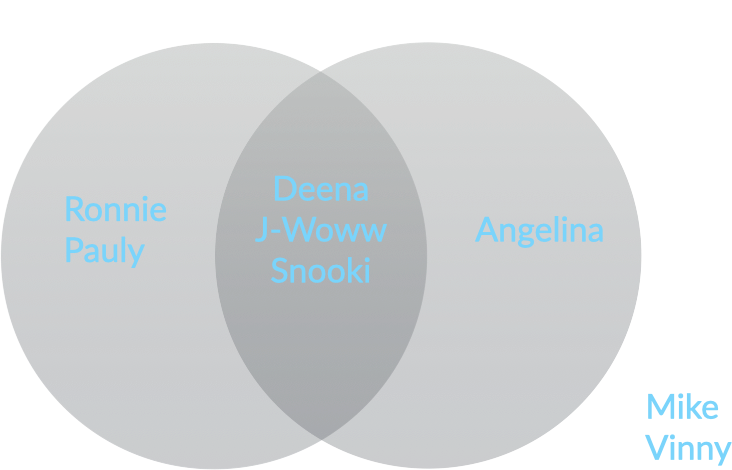
\includegraphics[width=3in]{venn}
      \end{center}
      
      \begin{align*}
        P(C|F) &= \frac{\text{Deena, J-Woww, Snooki}}{\text{Deena, J-Woww, Snooki, Angelina}} = \frac{3}{4} \\ 
               &= \frac{P(\text{$C$ and $F$})}{P(F)} = \frac{3/8}{4/8}
      \end{align*}
    \end{frame}


    \begin{frame}
      \begin{center}
        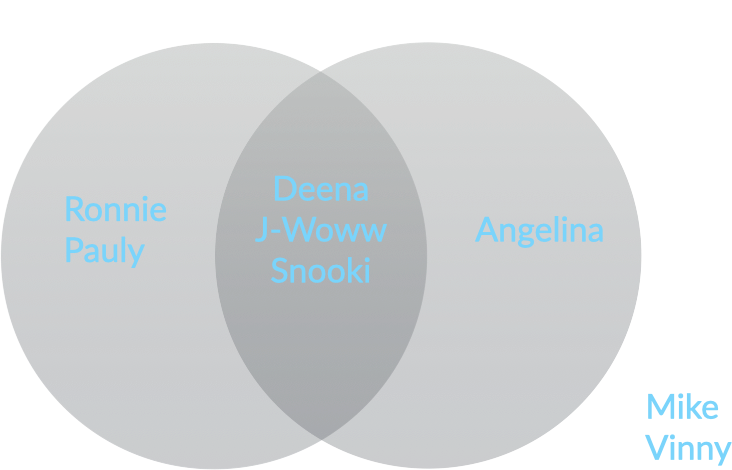
\includegraphics[width=3in]{venn}
      \end{center}
      
      $P(C|F) \neq P(F|C)$ --- they mean two different things:
      \begin{itemize}
        \item $P(C|F)$ is the proportion of feuding cast members that have children
        \item $P(F|C)$ is the proportion of cast members with children that are also feuding
      \end{itemize}
    \end{frame}


    \begin{frame}{Probability rules}
      \begin{enumerate}
        \item The chance of an event happening is between 0\% and 100\%, i.e. $0 \leq P(E) \leq 1$ for any event $E$.
        \item The probabilities for all possible outcomes put together add up to 1.
        \item The probability that something doesn’t happen is 100\% minus the probability that it does happen, i.e. $P(E^c) = 1-P(E)$.
        \item $P(\text{$A$ or $B$}) = P(A)+P(B) - P(\text{$A$ and $B$})$.
        \item $P(\text{$A$ and $B$}) = P(A)P(B|A)$.
      \end{enumerate}
    \end{frame}


    \begin{frame}{Two multiplication rules are really one}
      \begin{tabular}{ll}
        From last time: & $P(\text{$A$ and $B$}) = P(A)P(B)$, if $A$ and $B$ are independent \\
        From today:     & $P(\text{$A$ and $B$}) = P(A)P(B|A)$
      \end{tabular}

      \vspace{0.5in}\pause

      But these are really the same rule, since $P(B|A)=B$ exactly when $A$ and $B$ are independent! 

      \vspace{0.3in}\pause
      
      This is also how you can check if two events are independent: just check if $P(A)P(B)=P(\text{$A$ and $B$})$.
    \end{frame}

    \begin{frame}[fragile]{Reading conditional probabilities off of contingency tables}
      $P( \text{survived}|\text{female})$ is the proportion of women that survived:
\begin{knitrout}
\definecolor{shadecolor}{rgb}{0.969, 0.969, 0.969}\color{fgcolor}\begin{kframe}
\begin{alltt}
\hlkwd{prop.table}\hlstd{(}\hlkwd{table}\hlstd{(titanic}\hlopt{$}\hlstd{Sex, titanic}\hlopt{$}\hlstd{Survived),} \hlnum{1}\hlstd{)}
\end{alltt}
\begin{verbatim}
        
           No  Yes
  female 0.25 0.75
  male   0.79 0.21
\end{verbatim}
\end{kframe}
\end{knitrout}
      From this we can read off that $P(S|F) = 0.75$.
    \end{frame}

    \section{Probability trees}

    \begin{frame}{Probability trees}
      \begin{itemize}
        \item A way to visualize all joint ($P(\text{$A$ and $B$})$) and conditional ($P(B|A)$) probabilities for a particular situation
        \item A branch for each possible outcome
        \item At each level of the tree, assume the things to the left have already happened
        \item Each branch contains the probability of getting to that branch, conditional on what is to its left
        \item The leaves of the tree represents probabilities of final outcomes
      \end{itemize}
    \end{frame}

    \begin{frame}
      \begin{center}
        \begin{tikzpicture}
        [
          grow                    = right,
          level 1/.style          = {sibling distance=11em, level distance=4em},
          level 2/.style          = {sibling distance=6em, level distance=16em},
          edge from parent/.style = {draw, -latex},
          every node/.style       = {font=\footnotesize},
          sloped
        ]
        \node [none] {}
          child {
            node [none] {}
            child {
              node [leaf] { $P(\text{$M$ \& 1st})$ }
              edge from parent node [above] {1st class}
              edge from parent node [below] {$P(\text{1st}|M)$}
            }
            child {
              node [leaf] { $P(\text{$M$ \& 2nd})$ }
              edge from parent node [above] {2nd class}
              edge from parent node [below] {$P(\text{2nd}|M)$}
            }
            child {
              node [leaf] { $P(\text{$M$ \& 3rd})$ }
              edge from parent node [above] {3rd class}
              edge from parent node [below] {$P(\text{3rd}|M)$}
            }
            edge from parent node [above] {male}
            edge from parent node [below] {$P(M)$}
          }
          child {
            node [none] {}
            child {
              node [leaf] { $P(\text{$F$ \& 1st})$ }
              edge from parent node [above] {1st class}
              edge from parent node [below] {$P(\text{1st}|F)$}
            }
            child {
              node [leaf] { $P(\text{$F$ \& 2nd})$ }
              edge from parent node [above] {2nd class}
              edge from parent node [below] {$P(\text{2nd}|F)$}
            }
            child {
              node [leaf] { $P(\text{$F$ \& 3rd})$ }
              edge from parent node [above] {3rd class}
              edge from parent node [below] {$P(\text{3rd}|F)$}
            }
            edge from parent node [above] {female}
            edge from parent node [below] {$P(F)$}
          };
        \end{tikzpicture}
      \end{center}
    \end{frame}


    \begin{frame}
      
      \begin{center}
        \begin{tikzpicture}
        [
          grow                    = right,
          level 1/.style          = {sibling distance=11em, level distance=4em},
          level 2/.style          = {sibling distance=6em, level distance=16em},
          edge from parent/.style = {draw, -latex},
          every node/.style       = {font=\footnotesize},
          sloped
        ]
        \node [none] {}
          child {
            node [none] {}
            child {
              node [leaf] { $P(\text{$M$ \& 1st})$ }
              edge from parent node [above] {1st class}
              edge from parent node [below] {$P(\text{1st}|M)$}
            }
            child {
              node [leaf] { $P(\text{$M$ \& 2nd})$ }
              edge from parent node [above] {2nd class}
              edge from parent node [below] {$P(\text{2nd}|M)$}
            }
            child {
              node [leaf] { $P(\text{$M$ \& 3rd})$ }
              edge from parent node [above] {3rd class}
              edge from parent node [below] {$P(\text{3rd}|M)$}
            }
            edge from parent node [above] {male}
            edge from parent node [below] {0.62}
          }
          child {
            node [none] {}
            child {
              node [leaf] { $P(\text{$F$ \& 1st})$ }
              edge from parent node [above] {1st class}
              edge from parent node [below] {$P(\text{1st}|F)$}
            }
            child {
              node [leaf] { $P(\text{$F$ \& 2nd})$ }
              edge from parent node [above] {2nd class}
              edge from parent node [below] {$P(\text{2nd}|F)$}
            }
            child {
              node [leaf] { 0.13 }
              edge from parent node [above] {3rd class}
              edge from parent node [below] {0.35}
            }
            edge from parent node [above] {female}
            edge from parent node [below] {0.38}
          };
        \end{tikzpicture}
      \end{center}
    \end{frame}


    \begin{frame}
      
      \begin{center}
        \begin{tikzpicture}
        [
          grow                    = right,
          level 1/.style          = {sibling distance=11em, level distance=4em},
          level 2/.style          = {sibling distance=5em, level distance=16em},
          edge from parent/.style = {draw, -latex},
          every node/.style       = {font=\footnotesize},
          sloped
        ]
        \node [none] {}
          child {
            node [none] {}
            child {
              node [leaf] { 0.17 }
              edge from parent node [above] {1st class}
              edge from parent node [below] {0.27}
            }
            child {
              node [leaf] { 0.17 }
              edge from parent node [above] {2nd class}
              edge from parent node [below] {0.27}
            }
            child {
              node [leaf] { 0.29 }
              edge from parent node [above] {3rd class}
              edge from parent node [below] {0.46}
            }
            edge from parent node [above] {male}
            edge from parent node [below] {0.62}
          }
          child {
            node [none] {}
            child {
              node [leaf] { 0.13 }
              edge from parent node [above] {1st class}
              edge from parent node [below] {0.35}
            }
            child {
              node [leaf] { 0.11 }
              edge from parent node [above] {2nd class}
              edge from parent node [below] {0.3}
            }
            child {
              node [leaf] { 0.13 }
              edge from parent node [above] {3rd class}
              edge from parent node [below] {0.35}
            }
            edge from parent node [above] {female}
            edge from parent node [below] {0.38}
          };
        \end{tikzpicture}
      \end{center}
    \end{frame}
  \end{darkframes}
\end{document}
